\hypertarget{criterion-6-facilities-and-infrastructure}{%
\chapter{Criterion 6: Facilities and Infrastructure}\label{criterion-6-facilities-and-infrastructure}}

% \hypertarget{section-criterion-6-2026-4}{%
% \section{\texorpdfstring{\protect\includegraphics[width=6.5in,height=1.71528in]{media/image1.png}}{}}\label{section-criterion-6-2026-4}}

\hypertarget{Academic Facilities}{%
\section{Academic Facilities}\label{details-of-learning-and-support-facilities}}

SEECS has a total of 36 classrooms, with an average seating capacity of around 45 students. SEECS is equipped with two lecture halls. The first lecture hall seating 120 students and the second hall accommodating 90 students. The classrooms are equipped with modern technology, such as projectors, smart podiums with multimedia,
computers, audio-visual and digital lecture recording system equipment (Fig.~\ref{fig:figure1}). The classrooms are also well-ventilated and have comfortable
seating arrangements (Fig.~\ref{fig:figure2}). The classrooms are also equipped with Wi-Fi access and other necessary resources for students to use during their
studies. Moreover, SEECS now has two floors in the new Academic Block-I, which has been operational since September 2025. 14 new classrooms and 3 teaching labs have
been operational in the new academic block. SEECS infrastructure is summarised in Table~\ref{tab:infrastructure1}.

SEECS has established a smart classroom with 55'' touchscreen LEDs, remote conference, thin clients for 30 students, an auto-tracking camera, and microphones. Figure~\ref{fig:figure3} shows the view of smart classroom located in PG Block, SEECS.

\begin{figure}[htbp]
    \centering
    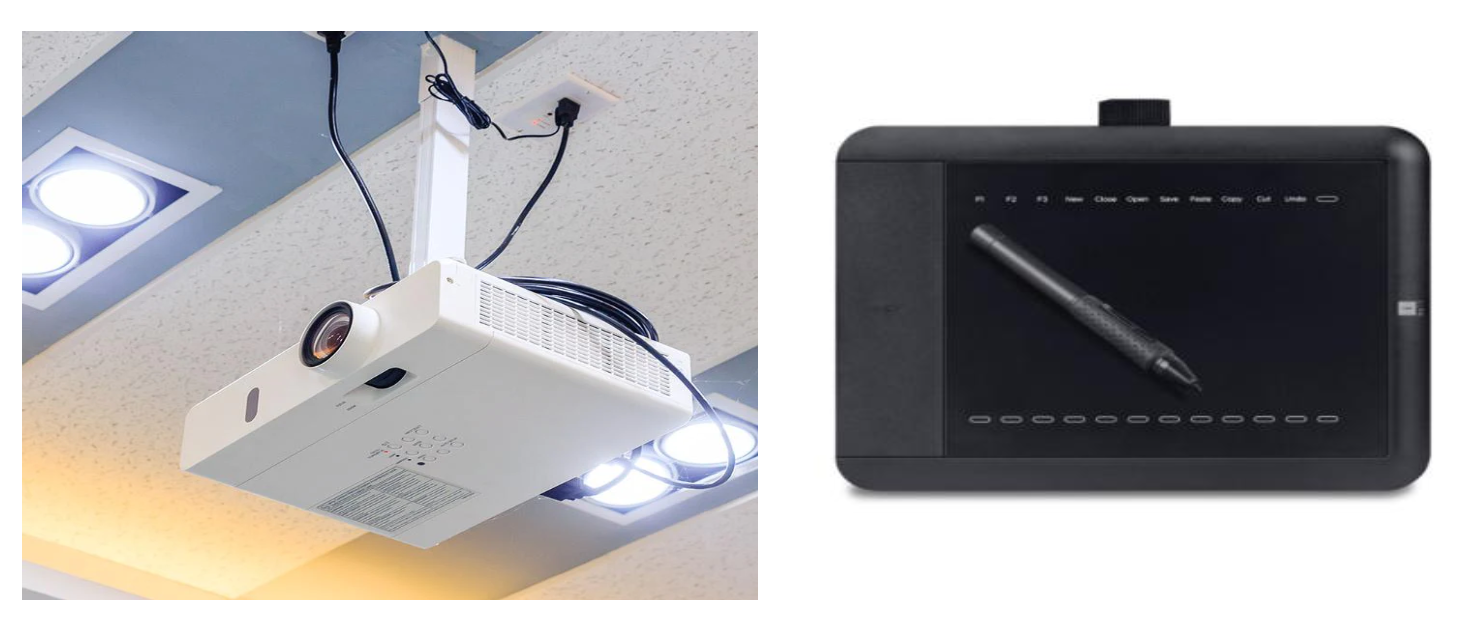
\includegraphics[width=0.85\textwidth]{images/criterion_6/media/1.png}
    \caption
    {Tools to Support Learning and Teaching.}
    \label{fig:figure1}
\end{figure}


\begin{figure}[H]
    \centering
    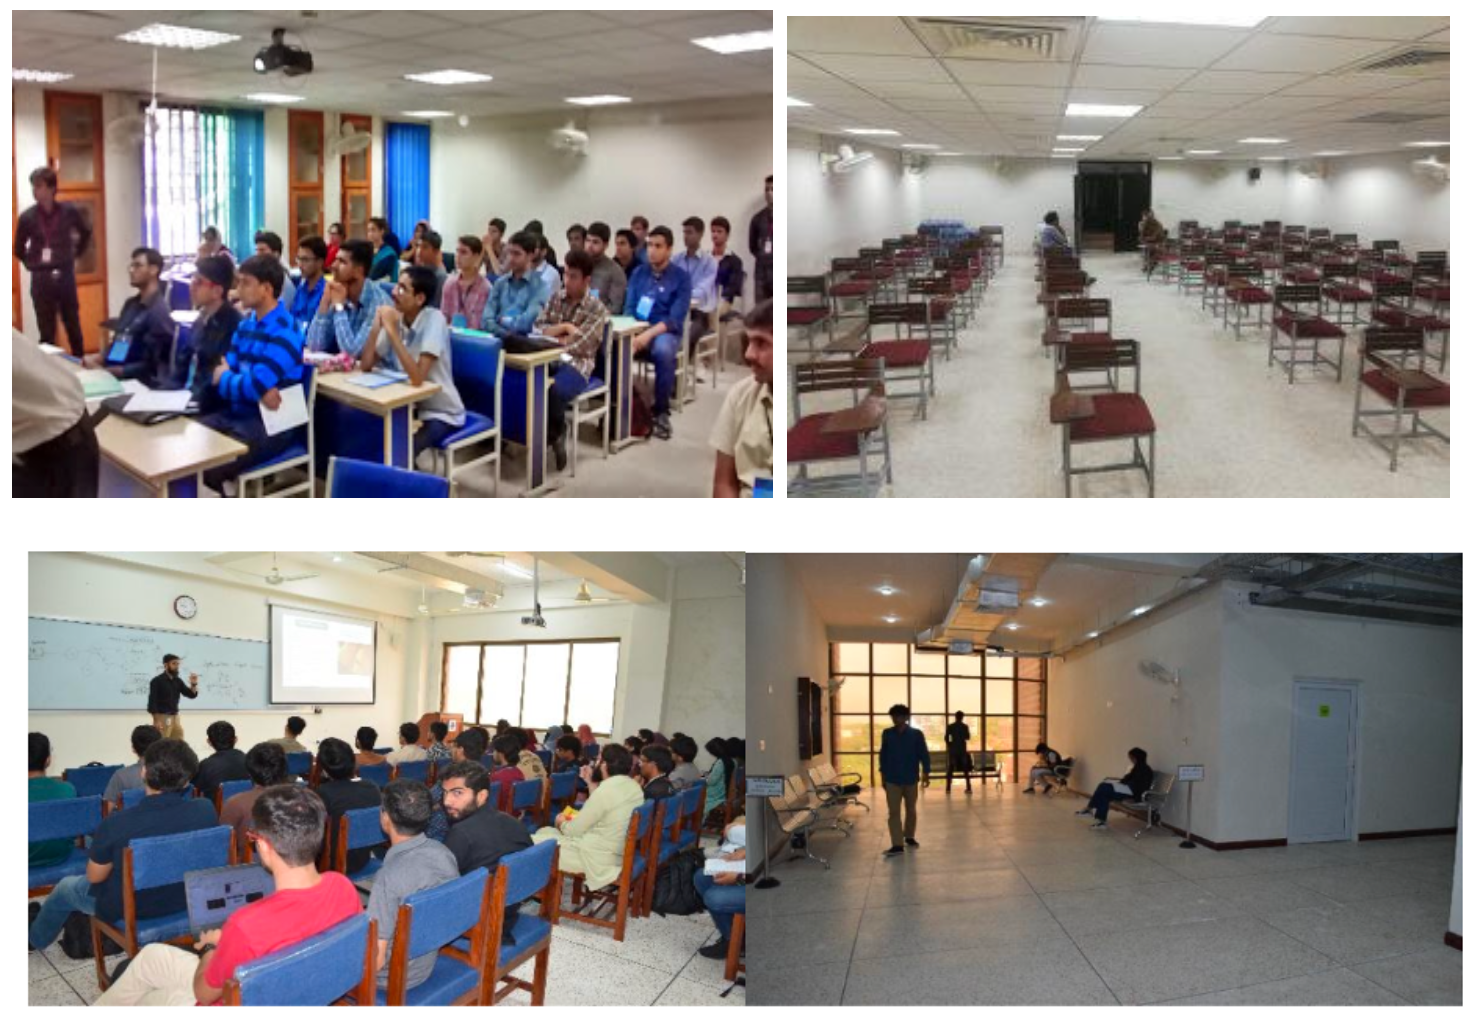
\includegraphics[width=1.0\textwidth]{images/criterion_6/media/2.png}
    \caption
    {Classrooms}
    \label{fig:figure2}
\end{figure}

\begin{table}[h]
  \centering
  \caption{SEECS infrastructure (existing blocks and New Academic Block)}
  \label{tab:infrastructure1}
  \small
  \begin{tabular}{|>{\raggedright\arraybackslash}p{0.39\textwidth}|>{\centering\arraybackslash}p{0.13\textwidth}|>{\centering\arraybackslash}p{0.15\textwidth}|>{\centering\arraybackslash}p{0.10\textwidth}|}
    \hline
    \textbf{Infrastructure} & \textbf{Existing blocks*} & \textbf{New Academic Block} & \textbf{Total} \\
    \hline
    Classrooms                            & 22      & 14      & 36       \\ \hline
    Offices -- Faculty / Officers         & 109     & 26      & 135      \\ \hline
    Principal / Assoc.\ Dean / HoD Offices & 6      & 10      & 16       \\ \hline
    Conference Rooms                      & 3       & 1       & 4        \\ \hline
    Faculty Lounges                       & 2       & 1       & 3        \\ \hline
    Common Rooms (male / female)          & 3       & 2       & 5        \\ \hline
    Exam Branch / Archive Room            & 1       & 1       & 2        \\ \hline
    Other Offices (IT/ACB/Admin/PA)       & 2/2/3/6 & 1/1/1/7 & 3/3/4/13 \\ \hline
  \end{tabular}

  \vspace{2pt}
  {\footnotesize *Existing blocks: UG/PG SEECS blocks, RIMMS and IAEC.\par}
\end{table}

\begin{figure}[H]
    \centering
    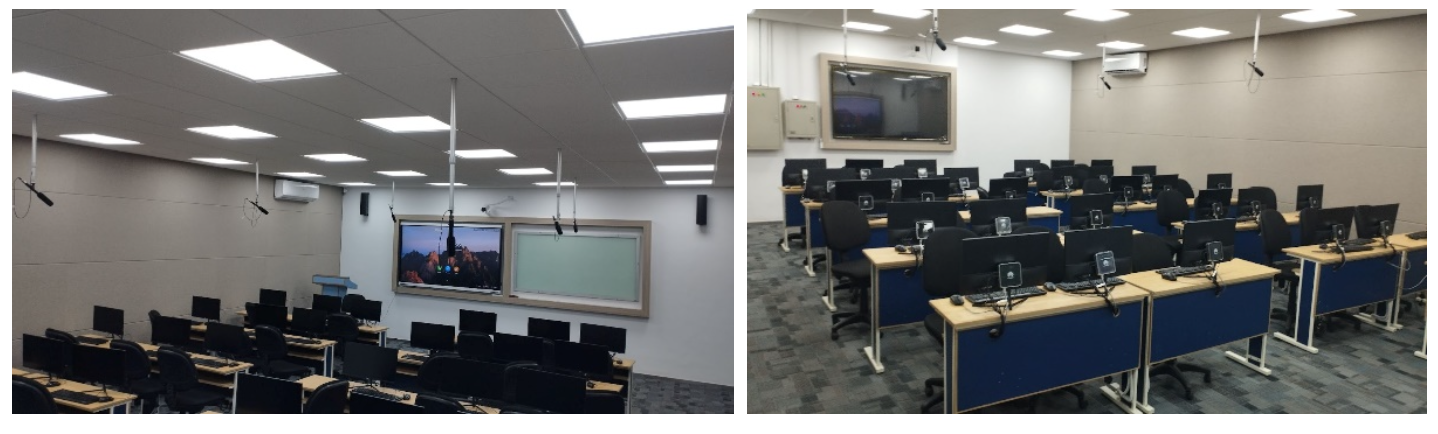
\includegraphics[width=1.0\textwidth]{images/criterion_6/media/3.png}
    \caption
    {Smart Classroom}
    \label{fig:figure3}
\end{figure}

\hypertarget{section-1}{%
% \section{\texorpdfstring{\protect\includegraphics[width=6.5in,height=2.44444in]{media/image8.png}}{}}\label{section-1}}
}

%\hypertarget{computer-facilities}{%
% \subsection{Computer Facilities}\label{computer-facilities}}

% Computer Facilities are available to all faculty members. Upon hiring, a faculty member is allocated a workstation. The equipment is upgraded as and when required depending on the requirements of the work conducted by the faculty member. 


\hypertarget{internet-facilities}{%
\subsection{Internet Facilities}\label{internet-facilities}}

Internet facility is available to all throughout the NUST campus. Internet facilities
are connected to PERN through NUST Campus Core Network with the bandwidth of
910 Mbps. NUST-SEECS also has a backup link of 7\,Mbps that is shared by some
specific research labs. The Internet at home facility is also available for those
faculty members who wish to use various resources at NUST-SEECS from their homes.
A Virtual Private Network (VPN) server is also hosted at NUST-SEECS so that faculty
can access computing resources housed at NUST-SEECS from their homes securely.
Reliable internet connectivity is available within the library to support access to
digital resources, online databases, and other academic services. Network performance
is regularly maintained to ensure uninterrupted access for students and faculty.


\hypertarget{laboratories}{%
\subsection{Laboratories}\label{laboratories}}

University lab facilities provide a range of resources to support students in their
academic pursuits. The facilities include 12 computer labs, 1 FYDP lab and 1 Basic
Electronics Lab. The computer labs are equipped with the latest hardware and
software, allowing students to access the internet, utilize specialized software,
complete assignments, or gain in-depth hands-on experience. The FYDP lab provides a
space for students to work on their final year design project, as well as receive
feedback from faculty and peers. The university lab facilities provide students with
the resources they need to succeed in their studies. The following laboratories are
available in SEECS, including teaching and research labs.

\begin{enumerate}[label=(\arabic*)]
  \item 12x Computer Labs
  \item 1x FYDP Lab (Final Year Design Projects Lab)
  \item 1x Basic Electronics Lab
  \item 11x Research Labs
\end{enumerate}

\hypertarget{computer-laboratories}{%
\subsubsection{Computing Laboratories (Teaching Laboratories)}\label{computer-laboratories}}
The institute has 12 computing laboratories and one Final Year Design Project (FYDP) Lab (Fig.~\ref{fig:figure4}). Computing Labs 1 and 2 have 48 and 51 systems installed
respectively. Computing Labs 3 to 9 on average have 40 systems, while Computing Labs 10 and 11 each have 41 systems installed. Computing Lab 12 is equipped with 35
systems, and the FYDP Computing Lab has 33 systems available for final-year project
work. Further details are provided in Annexure~\ref{annex:labs_labwork}.

\begin{figure}[htbp]
    \centering
    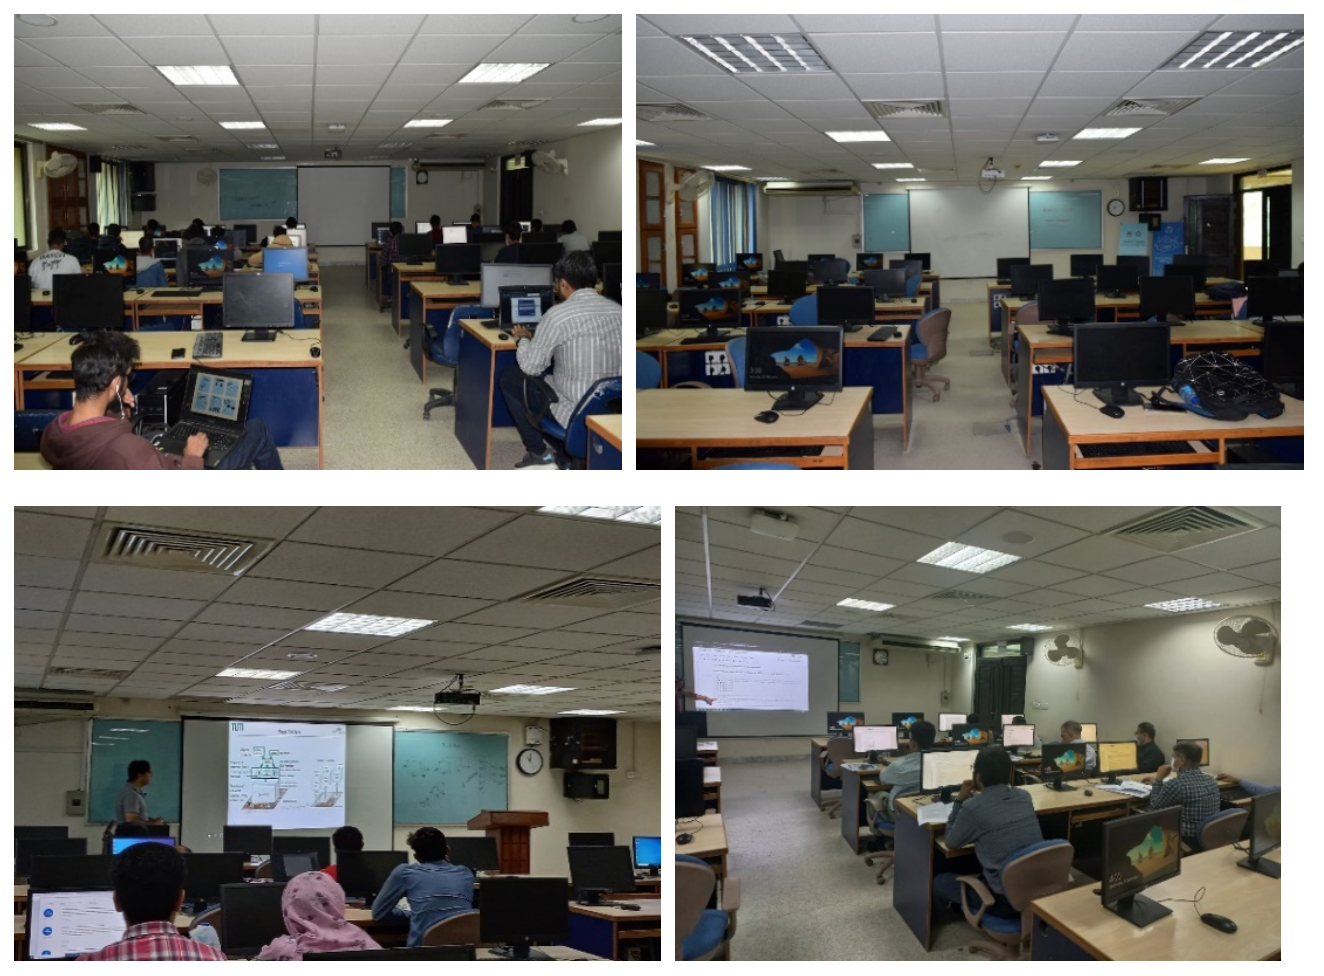
\includegraphics[width=1.0\textwidth]{images/criterion_6/media/4.png}
    \caption
    {Computer Labs}
    \label{fig:figure4}
\end{figure}


\hypertarget{research-laboratories}{%
\subsubsection{\texorpdfstring{Research Laboratories }{Research Laboratories }}\label{research-laboratories}}

The research laboratories provide a dedicated environment for conducting advanced research, experimentation, and innovation across diverse computing domains. The following research laboratories are present at SEECS:

\begin{enumerate}[noitemsep, topsep=0pt]
\def\labelenumi{(\alph{enumi})}

\item
  China-Pakistan Intelligent Systems (CPInS)

\item
  TUKL

\item
  High Performance Computing (HPC) Lab

\item
  Center for Research in Modeling, Simulation \& Vision (CRIMSON)

\item
  Knowledge-Based Systems (KBS) Lab

\item
  Walee-NUST Excellence Centre for Social \& Digital Media Technologies

\item
  Centre for Education Research and Practice (CERP)

\item
  Pak-Thai Digital Innovation Lab

\item
  Deep Learning Laboratory (DLL)

\item
  Software Modeling and Verification (SMV) Lab

\item
  NUST Staffordshire Creative AI Lab

\end{enumerate}

% New research labs such as the Internet of Things (IoT) lab and China-Pakistan Intelligent systems lab have been established after the last accreditation visit (Figure 7.5). This step has provided additional research opportunities and exposure to the UG students. We do believe in genuine improvements to fill any identified gaps. The above-stated additional facilities are substantial addition since the last accreditation visit.

% \begin{figure}[htbp]
%     \centering
%     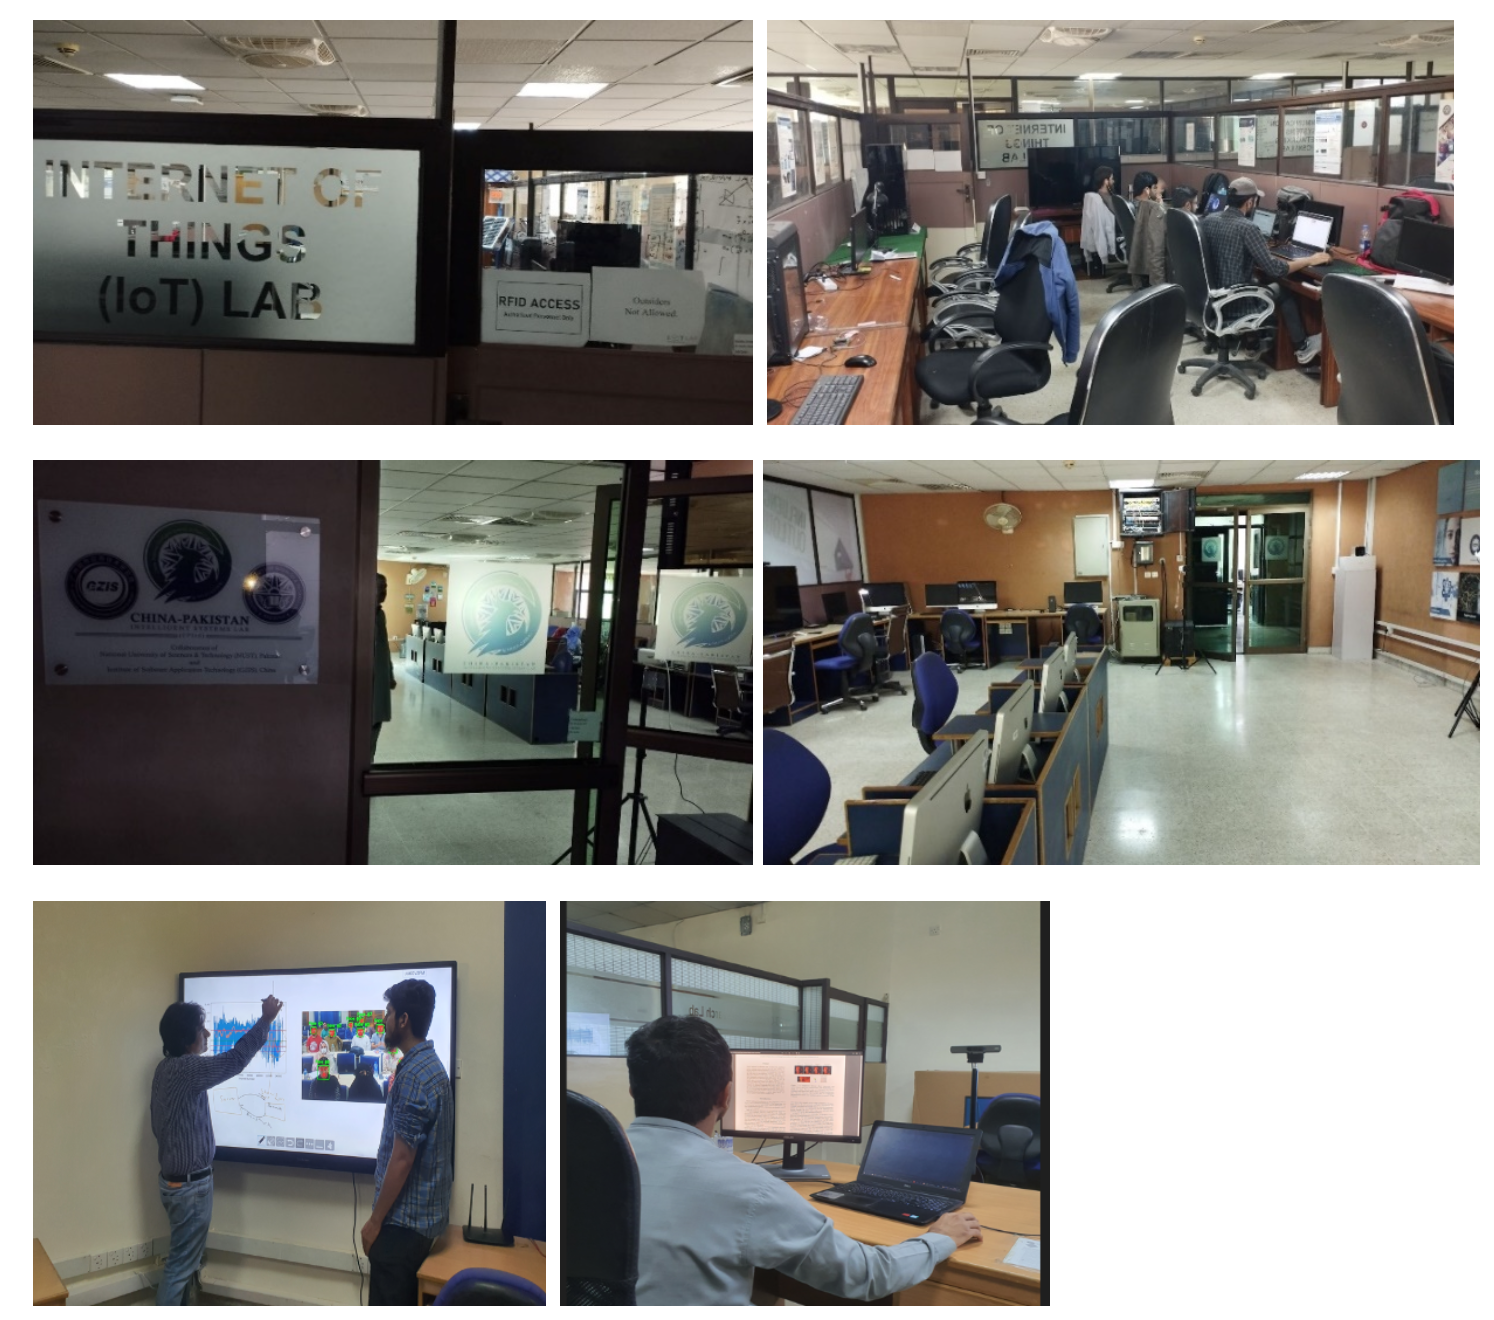
\includegraphics[width=1.0\textwidth]{images/criterion_6/media/6.png}
%     \caption
%     {Research Labs}
%     \label{fig:figure6}
% \end{figure}


\hypertarget{Conference and Seminar Halls }{%
\subsection{\texorpdfstring{Conference and Seminar Halls }{Conference and Seminar Halls }}\label{Conference and Seminar Halls}}

SEECS conference rooms and seminar halls provide a great facility for conducting
seminars, workshops, conferences, and hosting guest speakers. SEECS has 2 seminar
halls and 4 conference rooms. These rooms are equipped with the latest audio-visual
technology, comfortable seating, and ample space for large groups. They are also
equipped with whiteboards, projectors, and other necessary equipment for
presentations. Additionally, catering services are provided to attendees to ensure
that they are well-fed during the event. These rooms provide a professional and
comfortable environment for hosting events. Following seminar halls are available
at SEECS:

\begin{enumerate}
  \item SEECS (capacity 195)
  \item RIMMS (capacity 160)
\end{enumerate}

% TODO (dept): SE-SAR.xlsx says 1 of the 4 conference rooms is in the New Academic
% Block. Update the list below once the room/capacity is confirmed.
Moreover, following conference rooms are available:

\begin{enumerate}
  \item SEECS -- Faculty Block (capacity 25)
  \item SEECS -- PG Block (capacity 10)
  \item SEECS -- GRC (capacity 10)
  \item RIMMS (capacity 26)
\end{enumerate}

% \begin{figure}[htbp]
%     \centering
%     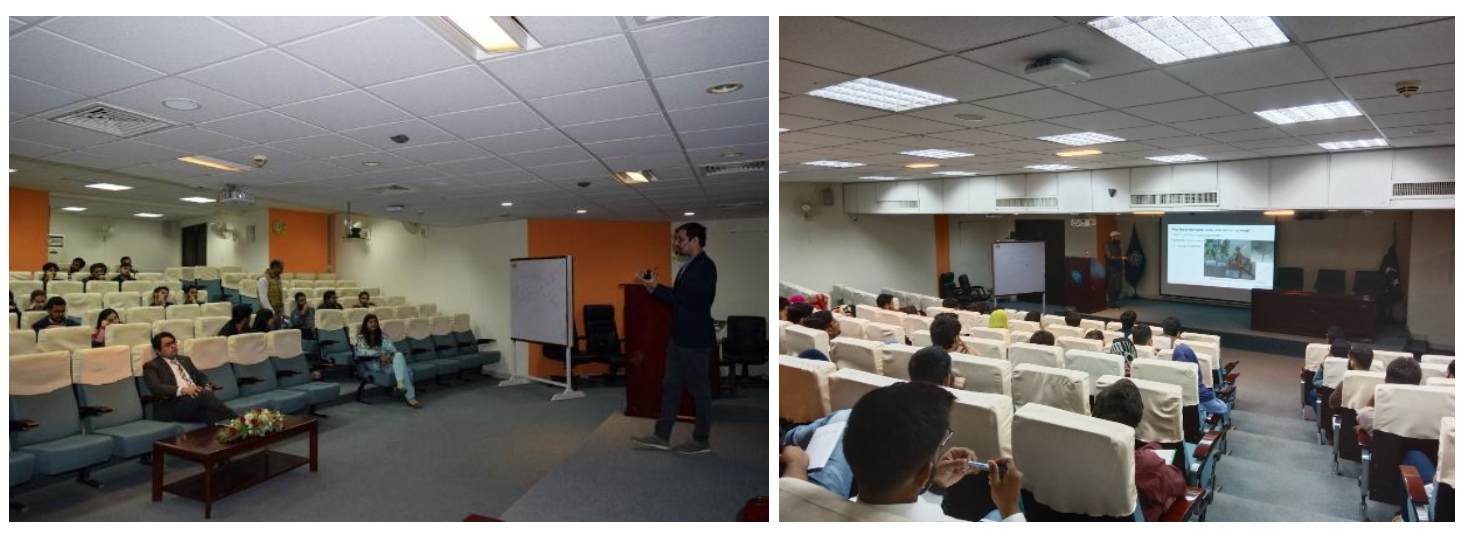
\includegraphics[width=1.0\textwidth]{images/criterion_6/media/9.png}
%     \caption
%     {Seminar Hall}
%     \label{fig:figure9}
% \end{figure}







\hypertarget{library}{%
\subsection{Library}\label{library}}

The NUST Central Library is a dynamic center of academic excellence, housing over
350,000 volumes across its main and institutional libraries. Spanning 42,907 sqft.,
this modern facility offers a serene, air-conditioned space for 570 readers,
accompanied by modern services like group study rooms, seminar halls, and cultural
hubs including the Lincoln and Chinese Corners, to support collaborative learning,
research activities, workshops, and academic events.

Spread across three floors, the library provides easy access to journals, circulation
collections, theses, and archives, empowering students, faculty, and researchers with
diverse resources to inspire learning, collaboration, and innovation. Additional
seating arrangements have been introduced to accommodate the increasing number of
library users, particularly during examination periods when daily footfall rises
significantly. To facilitate uninterrupted access to learning resources, the library
remains open seven days a week, with extended operating hours during examinations.
The University Central library facility is a comprehensive resource for students,
faculty, and staff as shown in Figure~\ref{fig:figure7}.

\begin{figure}[htbp]
    \centering
    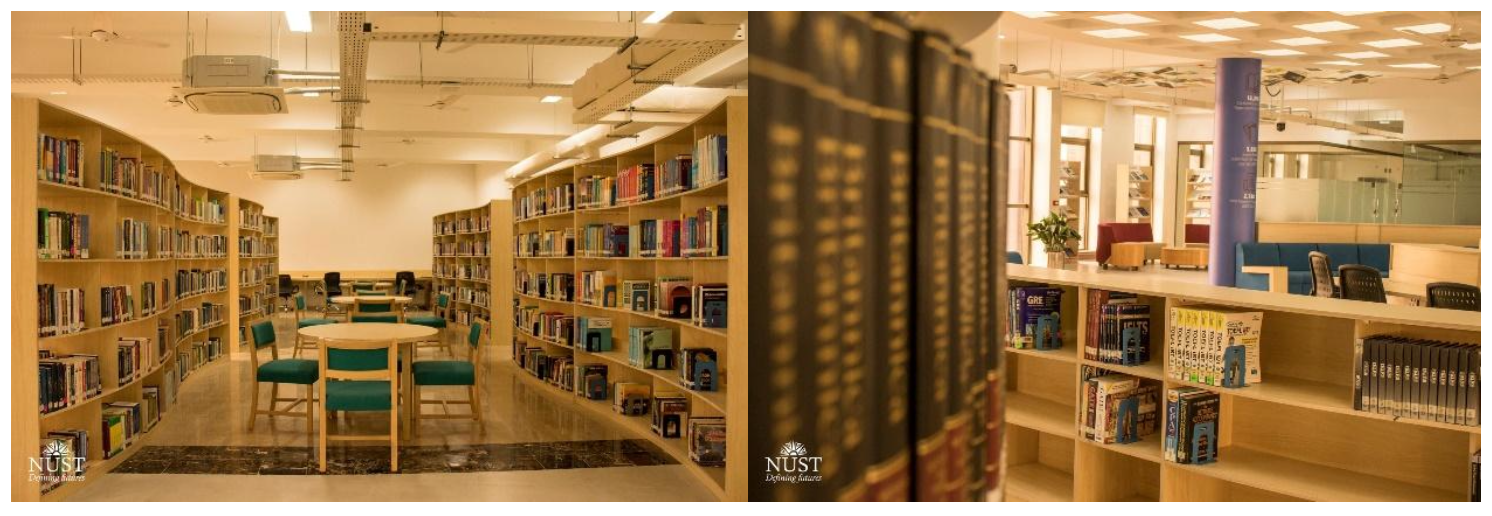
\includegraphics[width=1.0\textwidth]{images/criterion_6/media/7.png}
    \caption
    {NUST Central Library}
    \label{fig:figure7}
\end{figure}



\hypertarget{academic-library}{%
\subsubsection{Academic Library}\label{academic-library}}
The Central Library is well-equipped with an extensive collection of approximately 1,500 books related to Software Engineering and allied computing disciplines. This collection includes and is not limited to software engineering, programming, information technology, operating systems, web technologies, and data visualization. It supports the teaching, learning, and research needs of students, researchers, and faculty members.

% The collection covers a wide range of areas including software engineering principles, software design and development, software reliability, software reuse, embedded systems, programming languages, information technology, data visualization, operating systems, web technologies, and software tools. The library houses renowned titles such as Practical Software Reuse, Software Reliability Methods, Software Runaways: Monumental Software Disasters, The Java FAQ, Introduction to Information Technology, and several other reference books that support the teaching, learning, and research requirements of undergraduate and postgraduate students, researchers, and faculty members.

\subsubsection{Digital Library and Research Journals }\label{Digital ibrary}
The NUST Central library provides a seamless access to a wide range of educational resources to its faculty and students. A dedicated digital library containing a large collection of research papers, theses (23217), e-books (245), and project research archives are available through HEC. In addition to this, the central library subscribes to several other IEEE and ACM journals/magazines of international repute in hard-copy form which are readily available to the faculty and students. The university provides access to a comprehensive digital library through the Higher Education Commission (HEC), offering international research journals and scholarly databases in the domain of Software Engineering and related fields. The available resources include prestigious journals from Taylor and Francis and Wiley-Blackwell databases, including Software: Practice and Experience, Software Testing, Verification and Reliability, Journal of Software: Evolution and Process, Concurrency and Computation: Practice and Experience, Scientific Programming, Enterprise Information Systems, International Journal of Parallel, Emergent and Distributed Systems, Journal of Computer Information Systems, and Human Computer Interaction. These digital resources provide students and faculty with access to the latest advancements, research findings, and emerging trends in software engineering and computing technologies.


\subsubsection{Library Statistics }\label{library statistics}
The library provides all type of academics and research support to
students and faculty alike. Table~\ref{tab:library_inventory} provides the current inventory status.

\begingroup
\footnotesize
\setlength{\tabcolsep}{4pt}
\renewcommand{\arraystretch}{1.15}
\begin{longtable}{|>{\centering\arraybackslash}p{0.09\textwidth}|>{\raggedright\arraybackslash}p{0.53\textwidth}|>{\raggedright\arraybackslash}p{0.27\textwidth}|}
\caption{Library's current inventory}
\label{tab:library_inventory}\\
\hline
\textbf{Sr. No.} & \textbf{Item Description} & \textbf{Quantity} \\
\hline
\endfirsthead

\hline
\textbf{Sr. No.} & \textbf{Item Description} & \textbf{Quantity} \\
\hline
\endhead

1 & Total Printed Books & 44,092 \\
\hline
2 & Books on Software Engineering & 1,498 \\
\hline
3 & Online Books (HEC Subscribed) & 50,000 \\
\hline
4 & Printed Magazines & 14 \\
\hline
5 & Online Journals (HEC Subscribed) & 10 Resources (4 Basic \& 6 Premium) \\
\hline

\end{longtable}
\endgroup

\subsubsection{Library Management and Repository System}
The NUST Library System utilizes KOHA as its Integrated Library Management System (ILMS) and DSpace as its Institutional Repository platform.
Both systems are periodically upgraded and customized to improve functionality, usability, security, and system performance.
Continuous efforts are being made to enhance resource discovery and facilitate seamless access to library collections through improved system integration. Free subscription of Coursera through HEC, which includes several specializations is available for the faculty and students.

% \begin{figure}[htbp]
%     \centering
%     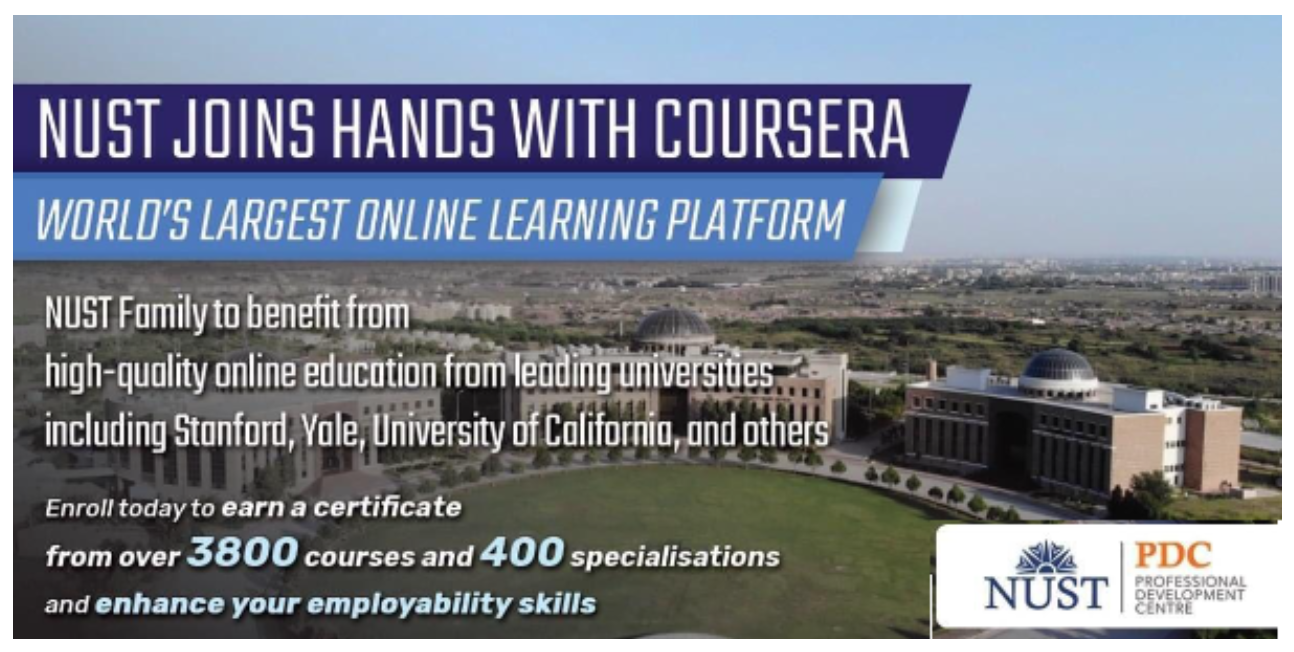
\includegraphics[width=1.0\textwidth]{images/criterion_6/media/8.png}
%     \caption
%     {Online Learning Platforms: Coursera}
%     \label{fig:figure8}
% \end{figure}



\subsubsection{NUST ConnectEd – Digital Learning Platform}\label{learning-platforms}

NUST ConnectEd is an interactive online learning platform designed to provide flexible and accessible learning opportunities through both self-paced and cohort-based courses. The platform offers pre-recorded learning content along with structured courses delivered by experienced NUST faculty. Courses are supported by supplementary learning materials, resources, and assessments, enabling learners to enhance their knowledge and skills while benefiting from a flexible and engaging digital learning environment.

In addition, NUST ConnectEd offers a Career Guidance Series aimed at supporting high school and undergraduate students in making informed academic and career choices. The series features guidance from experienced professionals and industry experts across diverse disciplines, emerging technologies, higher education, and professional pathways. It also provides practical guidance on educational opportunities, including topics such as postgraduate studies and international scholarship opportunities.
NUST ConnectEd can be accessed online through the official portal\footnote{https://connected.nust.edu.pk/}.

% Apart from these, Central Library is equipped with the state-of-the-art facilities such as bookable Group Study Rooms, Seminar Hall, Conference Room, computer terminals, high speed DSL and Wi-Fi Internet access and laptop points along with electric sockets for charging.

\hypertarget{support-facilities}{%
\section{Support Facilities}\label{support-facilities}}

\hypertarget{hostels}{%
\subsection{Hostels}\label{hostels}}

NUST provides comfortable and affordable on-campus accommodation for students, faculty, and employees. Fully furnished student hostels offer dining and essential amenities that support a focused academic environment. Faculty and employee residences provide a peaceful and secure setting, with nearby recreational facilities for adults and children. Figure~\ref{fig:figure10} shows the boys’ hostel building and rooms. NUST also offers dining facilities within hostels and faculty and officer accommodations. Cafeterias and tuck shops are located near academic buildings, offices, gymnasia, and residential blocks, while dedicated messes serve daily meals to faculty and officers.
Alongside campus-wide security, all hostels have protective boundary walls, security personnel, and dedicated staff. Each male and female hostel block is supervised by a hostel manager and a resident caretaker available around the clock.

\hypertarget{hostel-facilities}{%
\subsubsection{Hostel Facilities}\label{hostel-facilities}}

\begin{enumerate}[itemsep=1pt, topsep=2pt, parsep=0pt]
\item Fully furnished accommodation
\item Cubical / Bi-seater rooms with attached washroom
\item Bi-seaters / Tri-seater rooms with community Washroom
\item TV Room
\item Well-equipped Mess in each hostel
\item Laundry
\item Gymnasium
\item Badminton courts
\item Table Tennis
\item Billiard Board
\item Vending Machine
\item Electric Oven and Iron
\item Internet facility
\item Radiator Heating System
\item Medical cover for 24 hours
\item Shuttle service on Holidays
\end{enumerate}

\hypertarget{hostel-accommodation}{%
\subsubsection{Hostel Accommodation}\label{hostel-accommodation}}

Hostel Accommodation in the relevant category is strictly allotted according to the application seniority list. Hostels are well-maintained and provide all necessary facilities to make the students comfortable (Figure~\ref{fig:figure10}). The separately located hostels for males and females have been named after great Muslim scholars, as under:

\noindent\textbf{Hostels for Male Students}

\begin{enumerate}[itemsep=1pt, topsep=3pt, parsep=0pt]
    \item Rumi Hostels Block-I, II \& III -- PG Students
    \item Ghazali Hostels Block-I \& II -- UG Students
    \item Razi Hostels Block-I \& II -- UG Students
    \item Attar Hostels Block-I \& II -- UG Students
    \item Hajveri Hostel -- UG Students
    \item Zakariya Hostel -- UG Students
\end{enumerate}

\noindent\textbf{Hostels for Female Students}

\begin{enumerate}[itemsep=1pt, topsep=3pt, parsep=0pt]
    \item Fatima Hostels Block-I \& II -- PG Students
    \item Zainab Hostel -- UG Students
    \item Ayesha Hostel -- UG Students
    \item Khadija Hostel -- UG Students
    \item Amna Hostel -- UG Students
\end{enumerate}


%\textbf{Note}:~National UG Students in 1st to 3rd Semester will be allocated tri-seater accommodation in the hostels. 

% Annex AI contains more details on hostel facilities (Appendix~\ref{}).

\begin{figure}[htbp]
    \centering
    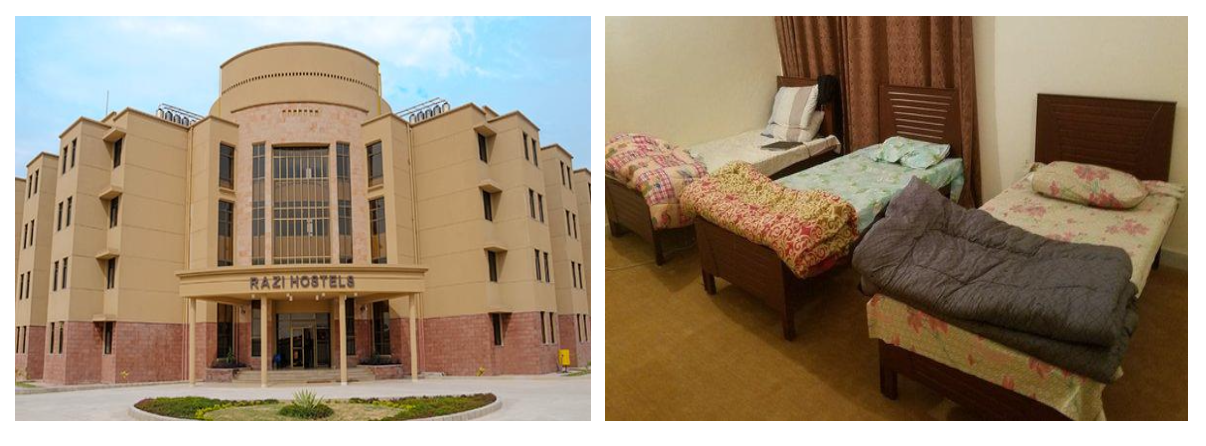
\includegraphics[width=1.0\textwidth]{images/criterion_6/media/10.png}
    \caption
    {Students hostel accommodation}
    \label{fig:figure10}
\end{figure}


\hypertarget{common-areas}{%
\subsection{Common Areas}\label{common-areas}}

By providing a comfortable and inviting atmosphere, common rooms can help foster a
sense of community among students and encourage them to stay connected with their
peers. SEECS offers a total of 5 common rooms which are equipped with comfortable
seating and tables. These spaces provide a place for students to socialize, study,
and take a break from their academic responsibilities.



\hypertarget{fitness-rooms}{%
\subsection{Fitness Rooms}\label{fitness-rooms}}

University fitness rooms provide students with access to a variety of exercise equipment and activities to help them stay healthy and fit. Fitness room is available at SEECS which includes a variety of cardio machines, strength training equipment, and free weights. The goal of SEECS fitness room is to provide students with the resources they need to maintain a healthy lifestyle.



\hypertarget{health-center}{%
\subsection{Health Center}\label{health-center}}

% On-campus medical facilities for students and staff is the most important service a university must provide to ensure the health and well-being of its employees and students. NUST Medical Centre provides health services, including 24/7 outpatient medical care for students and staff completely free of cost for everyone on campus. It also arranges inpatient medical cover in affiliated hospitals, while promoting activities for general wellbeing of NUST community (Figure 7.10).

% The medical center consists of at least two on-duty medical officers, nurses, staff, and round-the-clock emergency health-care services with ambulances. These free of cost medical facilities are available on all the seven campuses of NUST all over Pakistan. Other than these facilities, health insurance for staff and students has also been provided through subsidized insurance packages.

NUST Medical Centre provides free, 24/7 outpatient and emergency care for students and staff, supported by medical officers, nurses, and ambulance services. It also arranges inpatient care at affiliated hospitals and promotes community well-being (Figure~\ref{fig:figure11}).
Free medical services are available across all seven NUST campuses in Pakistan, complemented by subsidized health insurance packages for students and staff.
\begin{figure}[htbp]
    \centering
    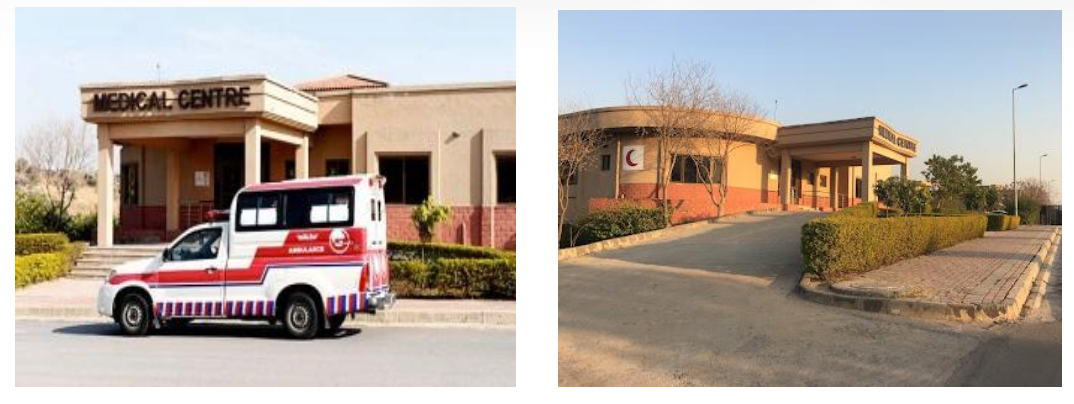
\includegraphics[width=1.0\textwidth]{images/criterion_6/media/11.png}
    \caption
    {NUST Medical Center (NMC)}
    \label{fig:figure11}
\end{figure}

\hypertarget{student-center}{%
\subsection{Student Center}\label{student-center}}

% The Student Center operates under the auspices of Student Affairs Directorate. The Center renders multiple services to NUST students as delineated below:

% \begin{enumerate}
% \def\labelenumi{\arabic{enumi}.}
% \item
%   Coordinates/ facilitates activities of all the University Clubs and Societies. The conduct of co-curricular activities through these forums enables students to enhance their mental abilities and prepare themselves for the daunting challenges of the future.
% \item
%   Runs a publications section comprising a team of editors and student editors, for publishing the University's monthly newsletter - NUSTNEWS, the annual bilingual literary magazine -- THE NUSTIAN, and a yearly publication NUSTXTRA, which exclusively covers both on- and off-campus co-curricular activities of the students. The Publications section also keeps liaison with HEC Publications Directorate for proper coverage of NUST events in its publications such as HEC newsletter- News \& Views. In addition to this, the publications department also covers the University events for publishing in the national and international press.
% \item
%   Houses a Fiction Library with a rich collection of literary works in both Urdu and English languages. The students enjoy leisure time from their tough academic routines, reading books of their choices. These books give them an insight into different meanings of and perspectives on life through the prism of veritable intellectual masterpieces.
% \item
%   Deals with discipline matters of students, as and when referred to student affairs (SA) Directorate by NUST institutions. Director Student Affairs heads the Discipline Committee.
% \item
%   Acts as a Front Office for processing all student related affairs/ queries, i.e., degrees, transcripts, refunds, scholarships etc.
% \item
%   Houses the Secretariat of Pakistan Chapter of The Talloires Network, PCTN. The Chapter promotes civic engagement in the higher education sector of Pakistan.
% \item
%   Provides facilities such as cafeteria, mini mart, stationery etc.
% \end{enumerate}


The Student Center operates under the Student Affairs Directorate renders multiple services to NUST students as delineated below:
\begin{enumerate}[noitemsep, topsep=0pt]
\item Coordinates university clubs, societies, and co-curricular activities to support students’ personal development and preparation for future challenges.

\item Manages university publications, including the monthly newsletter NUSTNEWS, the annual bilingual literary magazine THE NUSTIAN, and NUSTXTRA, which covers student co-curricular activities. It also coordinates coverage of university events in HEC publications and the national and international press.

\item Houses a Fiction Library offering Urdu and English literary works for leisure reading and intellectual enrichment.

\item Handles student disciplinary matters referred by NUST institutions, with the Director Student Affairs heading the Discipline Committee.

\item Serves as a front office for student queries and matters related to degrees, transcripts, refunds, and scholarships.

\item Houses the Secretariat of the Pakistan Chapter of the Talloires Network (PCTN), which promotes civic engagement in Pakistan’s higher education sector.

\item Provides amenities, including a cafeteria, mini mart, and stationery facilities.
\end{enumerate}

\subsection{NUST Student Support Services Centre (S3C)}
NUST Student Support Services Centre (S3C) is a new initiative which is centralized, one-window facilitation platform designed to streamline student requests and support services across campus.



\begin{enumerate}[noitemsep, topsep=0pt]
    \item \textbf{Student Help Desk}
    \begin{itemize}
        \item \textbf{Primary Function:} General queries, campus life facilitation, and academic enrollment assistance.
  %      \item \textbf{Phone Numbers:} \\+92-51-90851689 \textbar\ +92-51-90851699
  %      \item \textbf{Email:} \texttt{studenthelpdesk@nust.edu.pk}
    \end{itemize}

    \item \textbf{Center for Counseling and Career Advisory (C3A)}
    \begin{itemize}
        \item \textbf{Primary Function:} Professional mental health counselling, personal development workshops, and career guidance.
    \end{itemize}

    \item \textbf{Hostel Management}
    \begin{itemize}
        \item \textbf{Primary Function:} On-campus lodging, room allocations, and residential student affairs.
    %    \item \textbf{Male Hostels (Assistant Director):} +92-51-90851509
    %    \item \textbf{Female Hostels (Assistant Director):} +92-51-90851527
    \end{itemize}

    \item \textbf{Fee Affairs}
    \begin{itemize}
        \item \textbf{Primary Function:} Tuition management, installment schedules, and fee refund processing.
    \end{itemize}
\end{enumerate}

\subsection{Centre for Counselling and Career Advisory (C3A)}

The Centre for Counselling and Career Advisory (C3A) provides professional counselling services to support the mental health and well-being of NUST students, faculty, staff, and their families. The centre offers confidential counselling for educational, social, emotional, and psychological concerns that may affect personal or professional development. C3A is staffed by qualified psychologists and counsellors who provide individual and group counselling, consultation services, psychological assessments, psycho-educational programmes, training sessions, and workshops. Standardized psychological assessments, including Intelligence Quotient (IQ), Emotional Quotient (EQ), personality, aptitude, career interest, stress, anxiety, and depression tests, are available to promote the overall well-being and personal development of the university community.

\subsection{Career Development Centre (CDC)}

The Career Development Centre (CDC) is dedicated to enhancing students' employability by developing the professional and interpersonal skills required in today's competitive job market. The centre offers career development programmes, training modules, networking events, career counselling, employer engagement activities, curriculum support, and co-curricular initiatives to bridge the gap between academic learning and industry requirements. Through close collaboration with employers and the NUST Placement Office, the CDC equips students with the competencies necessary for successful career planning, employment, and professional growth.


\hypertarget{sport-and-recreational-facilities}{%
\section{Sports and Recreational Facilities}\label{sport-and-recreational-facilities}}

NUST affords an array of sports and other recreational facilities to its students, faculty, and staff. Sports infrastructure includes athletic tracks; cricket, hockey, and football grounds; various indoor sports facilities; gymnasia, etc. NUST has also recently established Pakistan's first university-based Horse-Riding Club and a one-of-a-kind Sports Complex, which includes swimming, archery, basketball, badminton, tennis, bowling, and other sports (Figure~\ref{fig:figure12}). The purpose of establishing such a facility is to invoke the urge for a healthy lifestyle among the NUST community, including students, alumni, faculty, staff, and their families. Moreover, there are also 80+ student-led Clubs and Societies across all campuses that inspire students to display and refine their dynamic literary, creative, and artistic abilities and aptitudes in the company of like-minded individuals.

\begin{figure}[htbp]
    \centering
    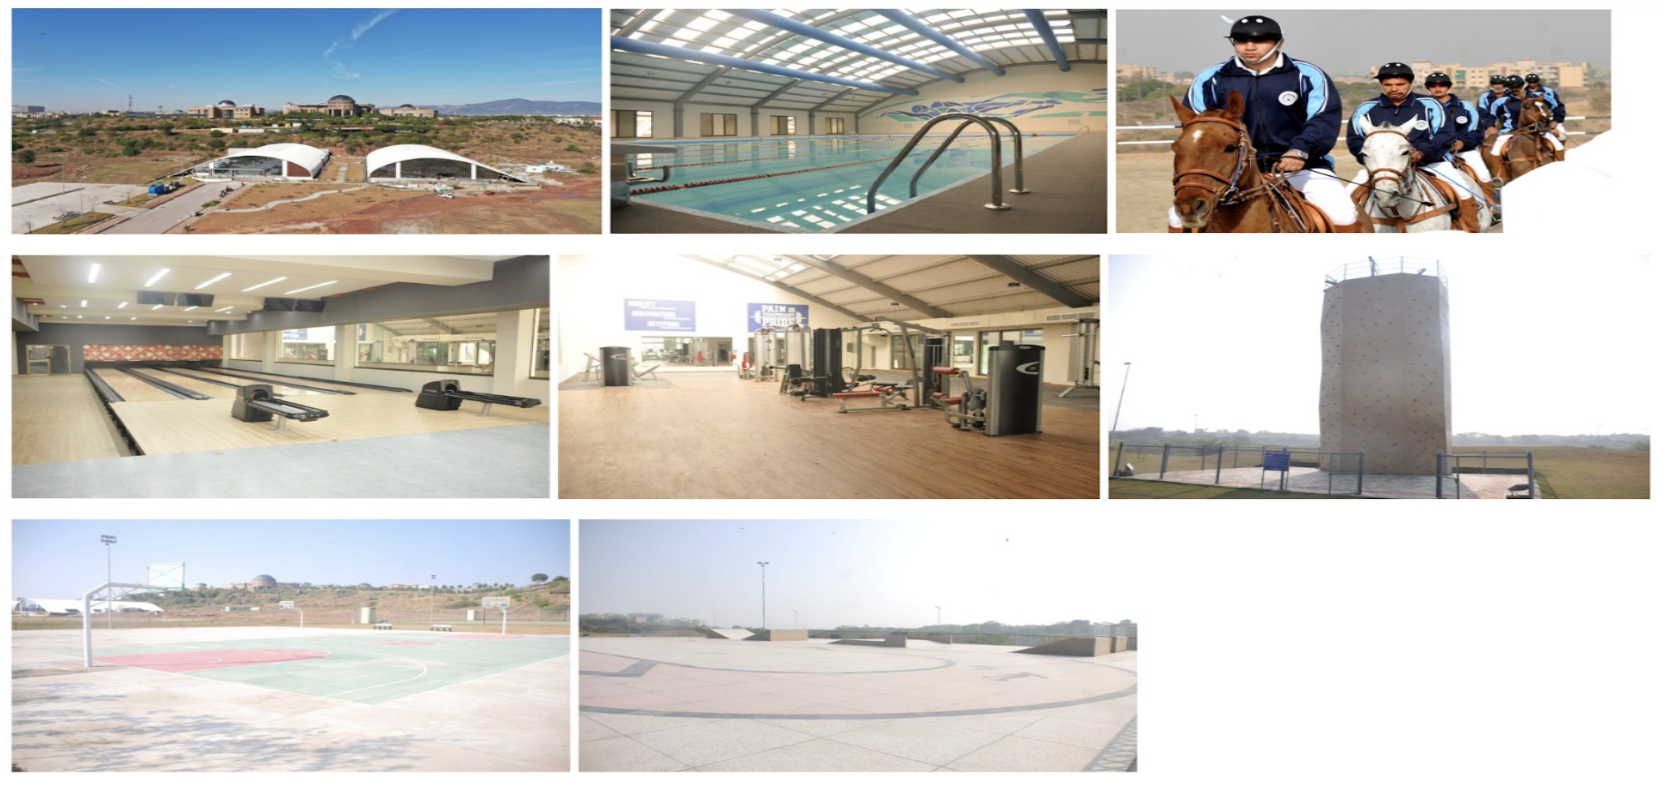
\includegraphics[width=1.0\textwidth]{images/criterion_6/media/12.png}
    \caption
    {Sports and recreational facilities}
    \label{fig:figure12}
\end{figure}


\hypertarget{cafes}{%
\subsection{Cafes}\label{cafes}}

Aesthetically designed cafeterias and shopping complex (Concordia I and Concordia II) have been constructed in the northern and southern wings of the campus (Figure~\ref{fig:figure13}). The cafeteria provides an opportunity to the students to relax and enjoy their snacks and meals in a hygienic environment. Each shopping complex offers the following services:
\begin{itemize}[itemsep=1pt, topsep=2pt, parsep=0pt]
    \item Cafeteria
    \item Mini Mart
    \item Photo Shop
    \item Barber Shop
    \item Ladies' Shop (including Parlor)
    \item Computer Hardware Shop
    \item Cellular Shop
    \item Business Center Services
    \item Stationery Shop
    \item Dining/Function Halls
\end{itemize}

\begin{figure}[htbp]
    \centering
    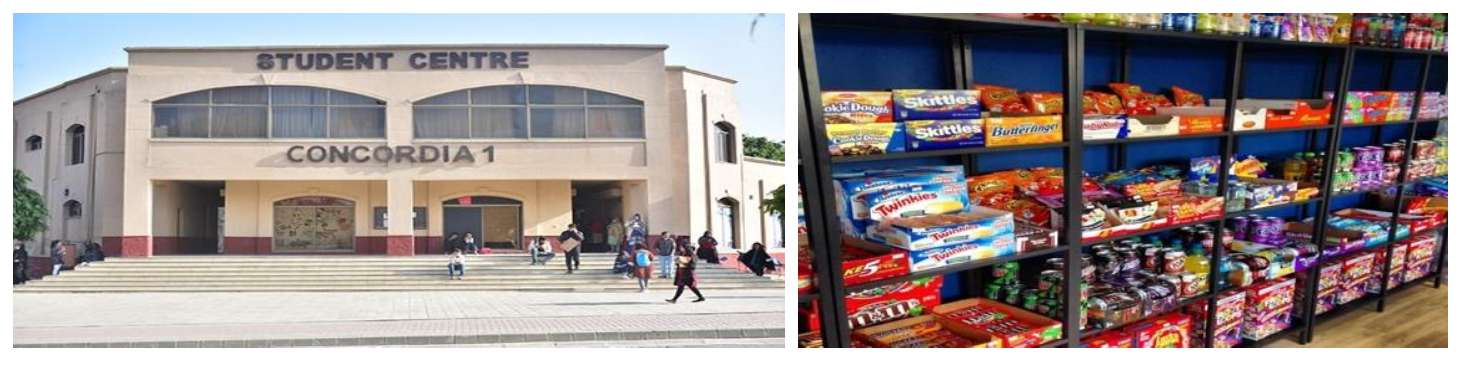
\includegraphics[width=1.0\textwidth]{images/criterion_6/media/13.png}
    \caption
    {Students cafeterias and tuck shops
}
    \label{fig:figure13}
\end{figure}


% \begin{figure}[htbp]
%     \centering
%     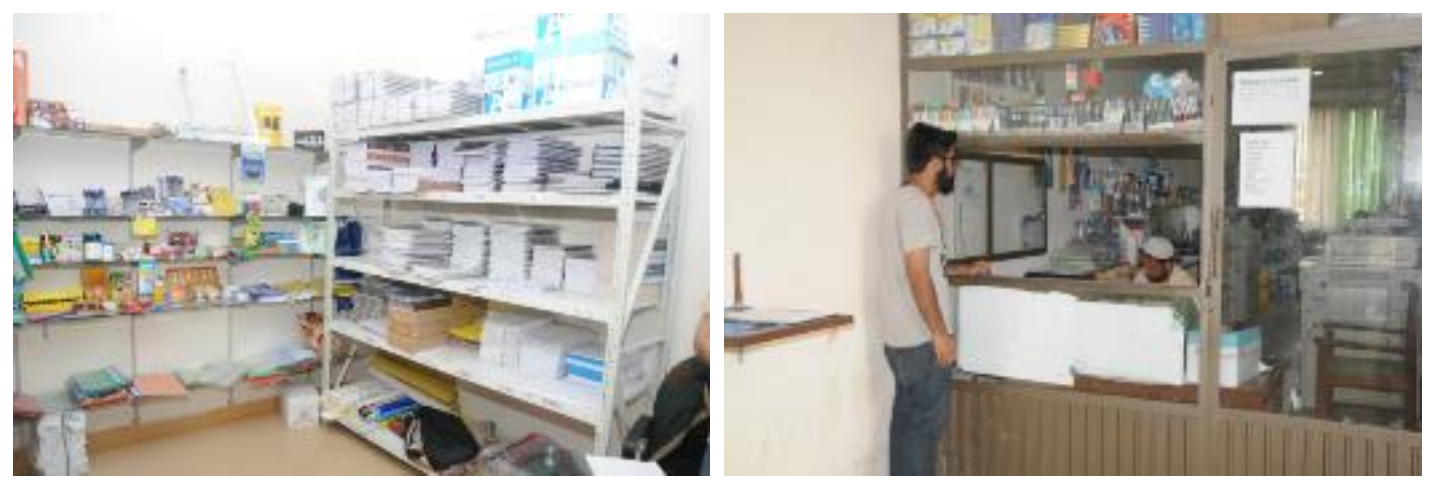
\includegraphics[width=1.0\textwidth]{images/criterion_6/media/14.png}
%     \caption
%     {Students café stationery shop
% }
%     \label{fig:figure14}
% \end{figure}


\hypertarget{transport-facilities}{%
\subsection{Transport Facilities}\label{transport-facilities}}

NUST has an elaborate and well-organized transport system to meet the requirements of students, faculty, and staff as shown in Figure~\ref{fig:figure15}. Special emphasis is on the environmentally friendly transport system. NUST runs a fleet of electric cars within its campus to minimize carbon emission. Electric cars are used as shuttle service between various locations within the campus, i.e., hostels to various School/Offices and from Gates to Schools/Hostels/Offices. NUST also has an elaborate transport system for pick and drop of students, faculty, and staff from all localities of the city with variable timings. Transport is also made available to facilitate students for industrial visits, research projects, club activities, society/community initiatives, awareness walks and excursion trips.

\begin{figure}[htbp]
    \centering
    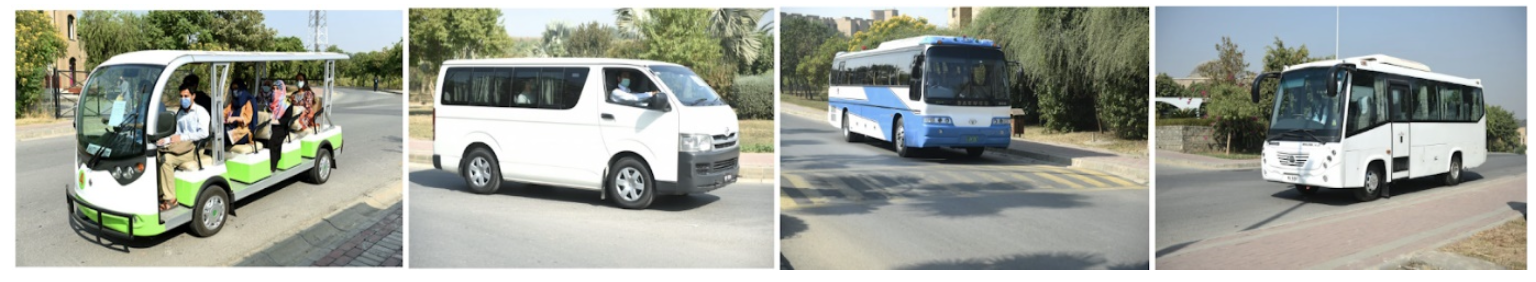
\includegraphics[width=1.0\textwidth]{images/criterion_6/media/15.png}
    \caption
    {NUST Transport Facility
}
    \label{fig:figure15}
\end{figure}


\subsection{Clubs and Societies}

With 44 clubs and societies, comprehensive sports facilities, recreational activities, and mega events, NUST provides students with opportunities to grow, explore, and experience life beyond academics. These activities not only offer a healthy balance to academic life but also encourage leadership, teamwork, and community engagement.

The major clubs and recreational facilities at NUST include:

\begin{itemize}[itemsep=1pt, topsep=2pt, parsep=0pt]
    \item NUST Bowling Alley
    \item NUST Horse Riding Club
    \item NUST Gyms and Swimming Pool
    \item NUST Hiking, Wall Climbing \& Excursion Club
    \item NUST Archery \& Pistol Club
    \item NUST Social Events and Societies
    \item NUST Community Services Club
\end{itemize}

Some of the main clubs and student organizations at SEECS are:

\begin{itemize}[itemsep=1pt, topsep=2pt, parsep=0pt]
    \item NUST Fitness Club (NFS)
    \item NUST Excursion Club (NXC)
    \item NUST Entrepreneurs Club (NEC)
    \item Institute of Electrical and Electronics Engineers (IEEE) Student Branch
    \item NUST Hack Club (NHC)
    \item Student Government Association (SGA)
    \item Graduate \& Professional Student Government (GPSG)
    \item Association for Computing Machinery (ACM)
    \item Youth Entrepreneurial Society (YES)
    \item International Association for the Exchange of Students for Technical Experience (IAESTE)
    \item Youth Impact SEECS Chapter
    \item Computer Society of Pakistan (CSP)
\end{itemize}



\hypertarget{workplace-safety}{%
\section{Workplace Safety}\label{workplace-safety}}

Health and safety are a top priority for the department and strict workplace safety regulations are followed to ensure a safe environment for all. Safe laboratory practices require a safety-conscious attitude, knowledge of hazards, and awareness of their presence. It is a shared responsibility that requires full cooperation from everyone in the workplace, including students, instructors, and researchers who must follow safety precautions and procedures. Safety instructions and evacuation plans are prominently displayed, and students receive regular briefings. The department ensures that necessary safety equipment is readily available and in good working order. Users are also trained in the location and use of safety facilities such as fire extinguishers, showers, and emergency exit, as well as familiarizing themselves with safety precautions, procedures, potential hazards, and emergency procedures.


\subsection{Work, Health and Safety}

To promote a safe and healthy working environment, SEECS has implemented a Work, Health and Safety (WHS) induction programme for all new faculty members, staff, research students, visitors, and affiliates associated with the School. The induction familiarizes participants with the University's health and safety policies, emergency procedures, reporting mechanisms, and workplace responsibilities. In addition, at least one WHS awareness and training session is conducted every semester for faculty and staff to reinforce safe work practices and ensure compliance with institutional policies and national occupational safety requirements.

The key topics covered during the induction and training sessions include:

\begin{enumerate}
  \item General Work, Health and Safety (WHS) responsibilities in accordance with the
        University Policy.
  \item Procedures for reporting incidents, injuries, illnesses, and workplace hazards.
  \item Local consultation arrangements for WHS matters through the School Safety
        Committee.
  \item Contact information for Safety Officers, First Aid Officers, and Building
        Wardens.
  \item Contact details are provided for reporting maintenance issues relating to
        buildings and grounds using the University Web Help Desk/ICT and other
        portals\footnote{\url{https://seecs.nust.edu.pk/contact/}}.
  \item Overview of occupational safety and health (OSH) legislation and relevant
        safety regulations applicable in Pakistan.
\end{enumerate}

NUST also follows a university wide University Health, Safety and Environment Policy. 
Detailed guidelines of university policy and SEECS health and safety induction checklist are available in Appendix~\ref{annex:NUST healthsafetypolicy} and Appendix~\ref{annex:work health safety checklist} respectively.

\hypertarget{fire-safety}{%
\subsection{Fire Safety}\label{fire-safety}}

The administration is dedicated to providing and maintaining a safe and healthy work environment. A standard operating procedure (SOP) has been established to handle fire emergencies which includes the following measures:

\begin{enumerate}[noitemsep, topsep=0pt]
\item Designation of a Fire Safety Officer for SEECS.
\item Designation of Fire Marshals for each floor of the building.
\item Installation of a fire alarm system.
\item Availability of 26 fire extinguishers and first aid boxes throughout the institute's building.
\item Posting of evacuation plans at prominent locations, offices, and classrooms.
\item Two emergency exit doors on each floor for safe evacuation.
\item Clearly marked assembly points outside the building.
\item Display of emergency contact numbers on noticeboards.
\item Availability of the NUST Medical Centre and Fire Department on campus to respond to emergencies.
\item Fire-fighting drills conducted every semester to enhance the awareness and preparedness of students and staff (Figure~\ref{fire_drill}).
\end{enumerate}

\begin{figure}[t]
    \centering
    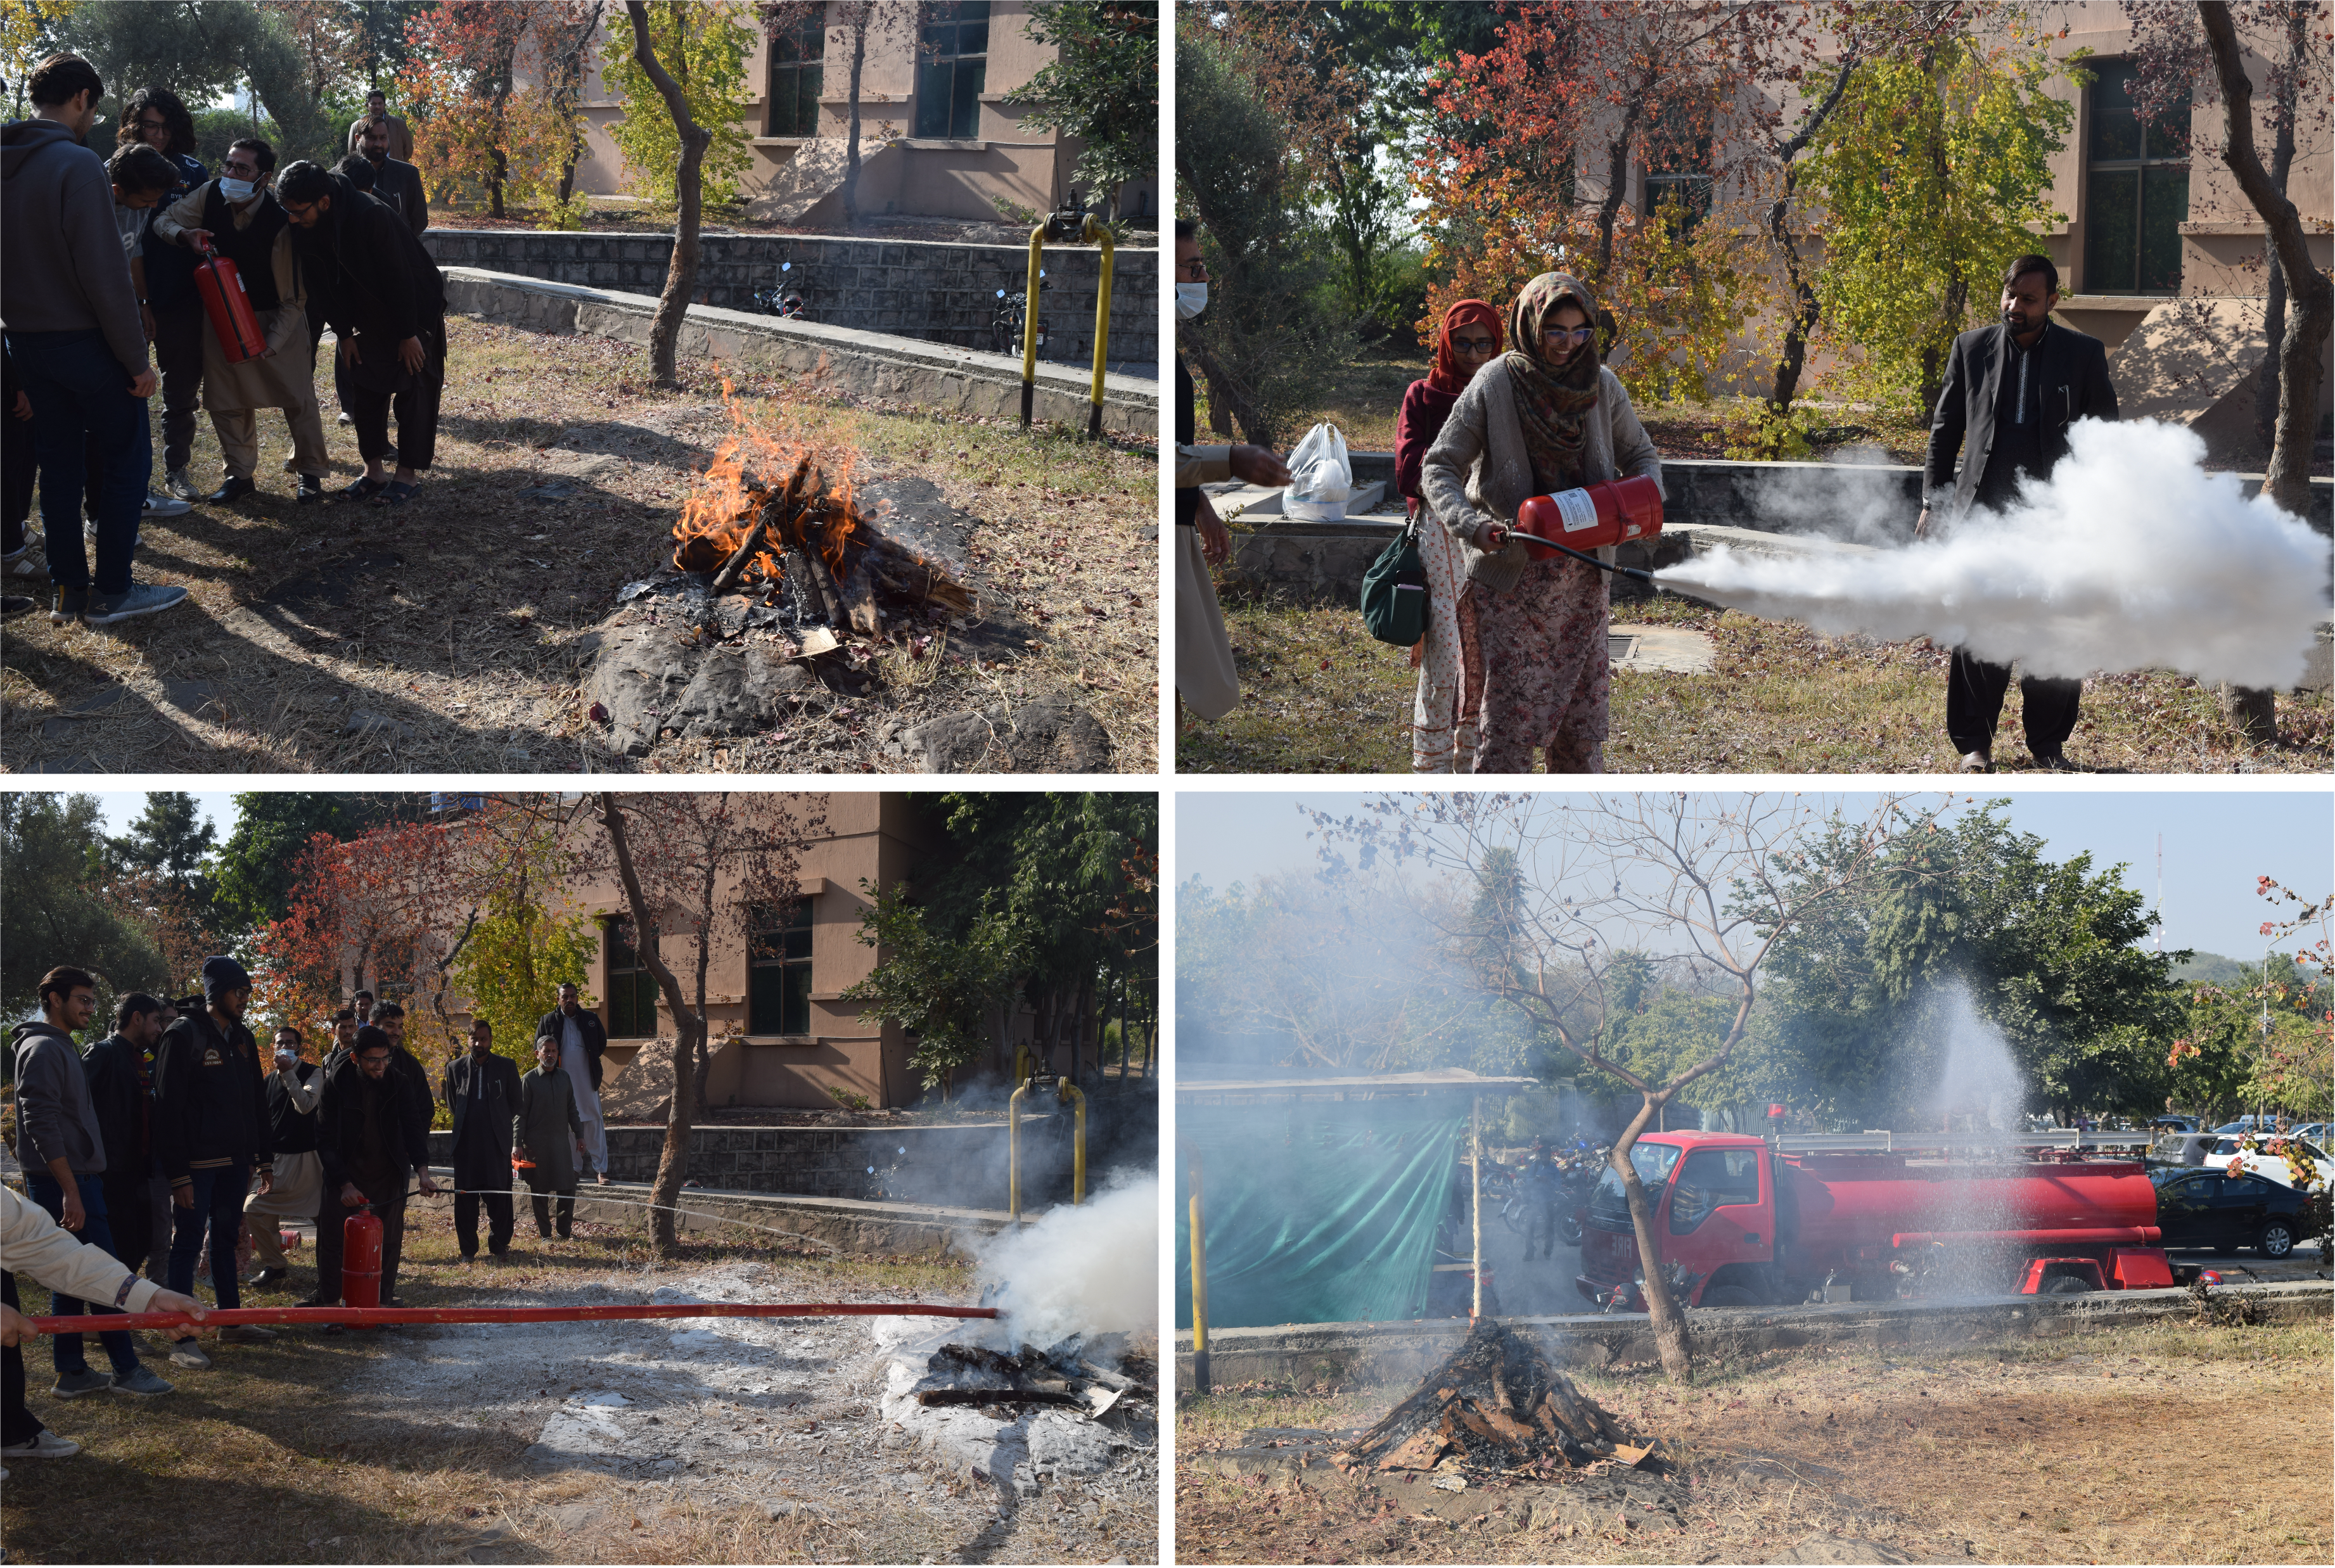
\includegraphics[width=1.0\textwidth]{images/criterion_6/media/img7.png}
    \caption{Fire drill exercise conducted at SEECS for awareness and preparedness of students and staff.}
    \label{fire_drill}
\end{figure}